\chapter{Cryptographic Preliminaries}

This chapter provides some cryptographic background information which is
relevant for the attribute-based credential systems which we describe in the
next chapters. In particular we focus on public-key cryptography in which a key
consists of a public an a private part. These key pairs are constructed such
that deriving the private part of the key from the public part is equivalent to
solving a computational problem that is considered extremely difficult.

\section{RSA Cryptography}\index{RSA}

In an RSA-based cryptosystem~\cite{RSA1978} a key pair consists a public part
$(n, e)$ and a private part $d$. The RSA modulus $n = p \cdot q$ is the product
of two primes $p$ and $q$ and the public exponent $e$ is a value that satisfies
$1 < e < \phi(n)$ and $gcd(e, \phi(n)) = 1$ where $\phi(n) = (p-1)(q-1)$ is
Euler's totient function\footnote{Euler's totient function $\phi(n)$ computes
the number of positive integers less then or equal to $n$ that are relatively
prime to $n$. An integer $k$ is relatively prime to $n$ if $gcd(k, n) = 1$.}.
The private exponent $d$ is a value that satisfies $1 < d < \phi(n)$ and
$e \cdot d = 1 \mod \phi(n)$, hence it can be computed as
$d = e^{-1} \mod \phi(n)$. When $p$ and $q$ are know, this computation is easy,
but computing $d$ based on just $n$ and $e$ is proved to be computationally
equivalent to determining the prime factors $p$ and $q$ of $n$, which is known
as the integer factorisation problem, a number-theoretic problem which is
considered intractable for large integers.

\subsection{Encryption Scheme}\index{RSA!encryption}

Such an RSA key pair can then be used to encrypt a message $m$ into an RSA
ciphertext $c = m^e \mod n$ using Algorithm~\ref{alg:RSA-encrypt}. Decryption
of such a ciphertext using Algorithm~\ref{alg:RSA-decrypt} is based on the fact
that
\begin{equation*}
  c^d = (m^e)^d = m^{e \cdot d} = m \mod n\text.
\end{equation*}

\begin{algorithm}[ht]
  \caption{RSA encryption.}
  \label{alg:RSA-encrypt}
  \addtolength{\baselineskip}{1mm}
  \begin{algorithmic}[1]
    \Function{RSA-encrypt}{$(n, e), m$}
      \State $c \gets m^e \mod n$
      \Return $c$
    \EndFunction
  \end{algorithmic}
\end{algorithm}
\begin{algorithm}[ht]
  \caption{RSA decryption.}
  \label{alg:RSA-decrypt}
  \addtolength{\baselineskip}{1mm}
  \begin{algorithmic}[1]
    \Function{RSA-decrypt}{$(n, e), c, d$}
      \State $m \gets c^d \mod n$
      \Return $m$
    \EndFunction
  \end{algorithmic}
\end{algorithm}

The problem of recovering the message $m$ based on the ciphertext $m^e \mod n$
and public key $(n, e)$ is known as the \emph{RSA problem}\index{RSA problem}.
This is equivalent to finding $e$th roots modulo $n$ which is assumed to be as
difficult as the integer factorisation problem\index{integer factorisation
problem}. Hence, the \emph{RSA assumption}\index{RSA assumpsion} states that
the probability that an attacker can solve the RSA problem is negligible.

\subsection{Signature Schemes}

In a similar fashion, this construction can also be used to create digital
signatures. To generate an RSA signature with Algorithm~\ref{alg:RSA-sign}, the
signer computes the message digest $h = \Call{Hash}{m}$ of the message to be
signed $m$ using a cryptographic hash function $\Call{Hash}{}$. This $h$, which
serves as a fingerprint of the original message, is then raised to the private
exponent. The result of this operation is the signature $s = h^d \mod n$ over
the message $m$.\index{RSA!signature}
Such an RSA signature can be verified using Algorithm~\ref{alg:RSA-verify}. The
verifier recovers the fingerprint $\hat{h} = s^e \mod n$ from the signature
value $s$ using the public exponent $e$ and checks whether this matches with the
message digest of the message $m$. If they match, the signature is valid,
otherwise the signature is invalid. The security of this RSA signature scheme is
also based on the RSA assumption.

\begin{algorithm}[H]
  \caption{RSA signature generation.}
  \label{alg:RSA-sign}
  \addtolength{\baselineskip}{1mm}
  \begin{algorithmic}[1]
    \Function{RSA-sign}{$(n, e), m, d$}
      \State $h \gets \Call{Hash}{m}$
      \State $s \gets h^d \mod n$
      \Return $s$
    \EndFunction
  \end{algorithmic}
\end{algorithm}
\begin{algorithm}[H]
  \caption{RSA signature verification.}
  \label{alg:RSA-verify}
  \addtolength{\baselineskip}{1mm}
  \begin{algorithmic}[1]
    \Function{RSA-verify}{$(n, e), m, s$}
      \State $\hat{h} \gets s^e \mod n$
      \If{$\hat{h} \neq \Call{Hash}{m}$}
        \Return \Call{Invalid}{}
      \EndIf
      \Return \Call{Valid}{}
    \EndFunction
  \end{algorithmic}
\end{algorithm}

Some other signature schemes based on the RSA cryptosystem, such as the
Camensich-Lysyanskaya scheme~\cite{CamenischLysyanskaya2003}
\index{Camenisch-Lysyansakay scheme} which is described
in Section~\ref{sec:CL-scheme}, only use the RSA modulus\index{RSA modulus} $n$ as the public part
of the key, whereas the private part consists of the primes $p$ and $q$. This
allows them to generate a fresh exponent $e$ for each signature which will then
become part of the signature. Since an attacker can now control both the
signature and the exponent, solving the RSA problem has become easier. Hence a
stronger assumption is needed. This \emph{strong RSA assumption}\index{strong RSA assumption} states that the
probability that an attacker can solve the RSA problem is negligible, even when
the attacker can chose the public exponent $e$.

\section{Discrete Logarithm Cryptography}

In a discrete logarithm-based cryptosystem~\cite{DH1976,ElGamal1985} a key pair
is accompanied with a description of the prime-order group in which the
computations take place. As an example we use $(p, q, g)$, where $p$ is a prime,
$q$ is a prime divisor of $p-1$, and $g$ is a generator, with order $q$, of a
subgroup of $\Z^*_p$. A private part of the key in such system is a random value
$x$ and the corresponding public part is $h = g^x \mod p$. The problem of
computing the private part $x = \log_g h$, based on the description of the group
$(p, q, g)$ and the public part $h$, is known as the \emph{discrete logarithm
problem}\index{discrete logarithm problem}.

\subsection{Key Agreement Scheme}\index{Diffie-Hellman key agreement}

The first discrete logarithm-based scheme was the key agreement scheme by Diffie
and Hellman~\cite{DH1976}. In this scheme a key pair as described above can be
used to compute a shared key with another party that uses the same group
parameters. To this end, both parties send their public key to each other and
compute the modular exponentiation of the received value and their private key,
as depicted in Figure~\ref{msc:DH}. The result of this computation can then be
used as a shared key\index{shared key} since
\begin{equation*}
  h_2^{x_1} = (g^{x_2})^{x_1} = g^{x_2 \cdot x_1}
  = k = g^{x_1 \cdot x_2} = (g^{x_1})^{x_2} = h_1^{x_2} \mod p
\end{equation*}
The problem of computing $k$, based on both public keys $h_1$ and $h_2$ and the
group description $(p, q, g)$, is assumed to be as difficult as the discrete
logarithm problem and is called the \emph{(computational) Diffie-Hellman problem}\index{Diffie-Hellman problem}. A related
problem is to determine whether a value $y$ is created using $h_1$ and $h_2$,
hence $y = g^{x_1 \cdot x_2}$, or not. This is known as the \emph{decisional
Diffie-Hellman problem}\index{decisional Diffie-Hellman problem}.

\begin{figure}[hb]
  \centering
  \includegraphics[scale=.45]{mscs/dh}
  \caption{Diffie-Hellman key agreement protocol.}
  \label{msc:DH}
\end{figure}

\subsection{Encryption}

The first encryption scheme based on discrete logarithms was proposed by
ElGamal~\cite{ElGamal1985}. In order to encrypt a message $m$, the user
generates a random value $r$ and commits to it by computing $c_1 = g^r \mod p$.
The value $r$ is then used to randomise the public key which is multiplied with
the message to obtain the encrypted message $c_2 = m \cdot h^r \mod p$. The
resulting ciphertext consists of both $c_1$ and $c_2$ (see Algorithm~\ref{alg:ElGamal-encrypt}.
In contrast to the RSA encryption scheme, the ElGamal encryption algorithm
produces a different ciphertext each time although the inputs remain the same.

The message $m$ can be recovered from a ciphertext $(c_1, c_2)$ by dividing
$c_2$ by $c_1^x = g^{r \cdot x} = h^r \mod p$, as described in Algorithm~\ref{alg:ElGamal-decrypt}. An attacker, who does not have
the private key $x$, must determine $h^r = g^{x \cdot r} \mod p$ based on the
public key $h = g^x \mod p$ and the commitment $c_1 = g^r \mod p$, that is, he
must solve the Diffie-Hellman problem.

\begin{algorithm}[t]
  \caption{ElGamal encryption.}
  \label{alg:ElGamal-encrypt}
  \addtolength{\baselineskip}{1mm}
  \begin{algorithmic}[1]
    \Function{ElGamal-encrypt}{$(p, q, g), h, m$}
      \State $r \gets \Call{Random}{}$
      \State $c_1 \gets g^r \mod p$
      \State $c_2 \gets m \cdot h^r \mod p$
      \Return $(c_1, c_2)$
    \EndFunction
  \end{algorithmic}
\end{algorithm}
\begin{algorithm}[t]
  \caption{ElGamal decryption.}
  \label{alg:ElGamal-decrypt}
  \addtolength{\baselineskip}{1mm}
  \begin{algorithmic}[1]
    \Function{ElGamal-decrypt}{$(p, q, g), (c_1, c_2), x$}
      \State $m \gets c_2 \cdot c_1^{-x} \mod p$
      \Return $m$
    \EndFunction
  \end{algorithmic}
\end{algorithm}

\subsection{Signatures}

Many signature schemes have been based on the discrete logarithm problem, for
example the Chaum-Pedersen scheme which is described in
Section~\ref{sec:CP-scheme}, but also the Digital Signature Algorithm (DSA),
which is part of the Digital Signature Standard of the United States government.
The digital signature algorithm, described in Algorithms~\ref{alg:DSA-sign}
and~\ref{alg:DSA-verify}, is similar to the first discrete logarithm-based
signature scheme proposed by ElGamal~\cite{ElGamal1985}. Like the encryption
scheme, the signature $(r, s)$ consists of two parts. The first is a commitment
on the randomisation value, whereas the second part commits to the fingerprint
$h$ of the message $m$ that is to be signed. This signature cannot be verified
directly, but is based on reconstructing the commitment value using the public
key of the signer and the fact that
\begin{equation*}
  k = s^{-1} \cdot (c + x \cdot r) \mod q\text.
\end{equation*}

\begin{algorithm}
  \caption{DSA signature generation.}
  \label{alg:DSA-sign}
  \addtolength{\baselineskip}{1mm}
  \begin{algorithmic}[1]
    \Function{DSA-sign}{$(p, q, g), m, x$}
      \State $r \gets 0$
      \While{$r = 0 \mod p$}
        \State $k \gets \Call{Random}{~}$
        \State $r \gets (g^k \mod p) \mod q$
      \EndWhile
      \State $c \gets \Call{Hash}{m}$
      \State $s \gets k^{-1} \cdot (c + x \cdot r) \mod q$
      \Return $(r, s)$
    \EndFunction
  \end{algorithmic}
\end{algorithm}
\begin{algorithm}
  \caption{DSA signature verification.}
  \label{alg:DSA-verify}
  \addtolength{\baselineskip}{1mm}
  \begin{algorithmic}[1]
    \Function{DSA-verify}{$(p, q, g), m, (r, s), h$}
      \State $c \gets \Call{Hash}{m}$
      \State $u \gets c \cdot s^{-1} \mod q$
      \State $v \gets r \cdot s^{-1} \mod q$
      \State $\hat{r} \gets (g^u \cdot h^v \mod p) \mod q$
      \If{$\hat{r} \neq r$}
        \Return \Call{Invalid}{}
      \EndIf
      \Return \Call{Valid}{}
    \EndFunction
  \end{algorithmic}
\end{algorithm}

\section{Elliptic Curve Cryptography}

In the previous section we described the discrete logarithm cryptography in a
setting of a prime order subgroup of $\Z^*_p$. These techniques can, however,
be applied to any finite cyclic group. Another popular setting for implementing
discrete logarithm systems is the elliptic curve setting which we describe below.

\subsection{Elliptic Curves}

Given a finite field $\F{q}$ containing $q$ elements, where $q$ is a prime
power, an elliptic curve $E$ over $\F{q}$ is defined by the equation
\begin{equation}\label{eqn:elliptic_curve}
  E: y^2 = x^3 + a \cdot x + b
\end{equation}
where $a, b \in \F{q}$ are the curve parameters that satisfy $4 \cdot a^3 + 27 \cdot b^2 \neq 0$.
The set of all points $P = (x, y)$ on this curve $E$ is denoted as
\begin{equation*}
  E(\F{q}) = \{ (x, y) \in \F{q} \times \F{q} : y^2 = x^3 + a \cdot x + b \}
                         \cup \{ \infty \}
\end{equation*}
where $\infty$ is a special point called the \emph{point at infinity}.


\begin{figure}[ht]
  \centering
  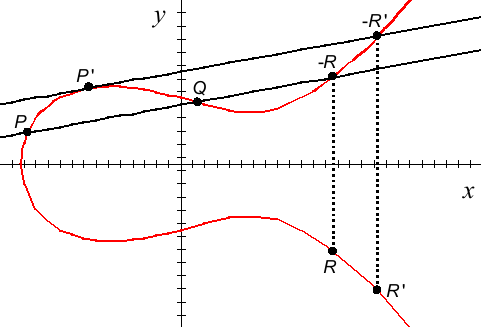
\includegraphics[scale=.4]{images/ec_math}
  \caption{Geometric visualisation of point addition ($R = P + Q$), point
    doubling ($R' = 2P'$) and point negation ($-R$) on an elliptic curve.}
  \label{fig:EC}
\end{figure}

On these points three basic operations can be defined: negation, addition and
doubling. These operations are detailed below and visualised geometrically in
Figure~\ref{fig:EC}.
\begin{enumerate}
  \item \emph{Point negation}, the \emph{negative} $R = -P$, of the point $P$
    is computed according to Algorithm~\ref{alg:ec_point_negation}.
    Geometrically, this is the reflection of point $P$ in the $x$-axis.
    \begin{algorithm}[H]
      \caption{Elliptic curve point negation: $R = -P$}
      \label{alg:ec_point_negation}

      \begin{algorithmic}[1]
        \Function{ECPointNegation}{$P$}
          \If{$P = \infty$}
            \Return $\infty$
          \EndIf

          \State $(x_P, y_P) \gets P$

          \Return $(x_P, -y_P)$
        \EndFunction
      \end{algorithmic}
    \end{algorithm}

  \item \emph{Point addition}, the \emph{sum} $R = P + Q$, of the points $P$
    and $Q$ is computed using Algorithm~\ref{alg:ec_point_addition}.
    In geometry, this is the reflection in the $x$-axis of the intersection of
    the curve and the line through the points $P$ and $Q$.
    \begin{algorithm}[H]
      \caption{Elliptic curve point addition: $R = P + Q$}
      \label{alg:ec_point_addition}

      \begin{algorithmic}[1]
        \Function{ECPointAddition}{$P$, $Q$}
          \If{$P = \infty$}
            \Return $Q$
          \EndIf
          \If{$P = Q$}
            \Return $2 \cdot P$
          \EndIf
          \If{$P = -Q$ or $Q = \infty$}
            \Return $\infty$
          \EndIf

          \State $(x_P, y_P) \gets P$
          \State $(x_Q, y_Q) \gets Q$

          \State $x \gets \left(\dfrac{y_Q - y_P}{x_Q - x_P}\right)^2 - x_P - x_Q \mod q$
          \State $y \gets \left(\dfrac{y_Q - y_P}{x_Q - x_P}\right) (x_P - x_R) - y_P \mod q$

          \Return $(x, y)$
        \EndFunction
      \end{algorithmic}
    \end{algorithm}

  \item \emph{Point doubling}, the \emph{double} $R = 2 \cdot P$ is computed
    using Algorithm~\ref{alg:ec_point_doubling}. Geometrically, this is the
    reflection in the $x$-axis of the intersection of the curve and the tangent
    line to the curve at the point $P$, see Figure~\ref{fig:EC}.
    \begin{algorithm}
      \caption{Elliptic curve point doubling: $R = 2 \cdot P$}
      \label{alg:ec_point_doubling}

      \begin{algorithmic}[1]
        \Function{ECPointDoubling}{$P$}
          \If{$P = \infty$}
            \Return $P$
          \EndIf

          \State $(x_P, y_P) \gets P$

          \State $x_R \gets \left(\dfrac{3 x_P^3 + a}{2 y_P}\right)^2 - 2 x_P \mod q$
          \State $y_R \gets \left(\dfrac{3 x_P^3 + a}{2 y_P}\right) (x_P - x_R) - y_P \mod q$

          \Return $(x_R, y_R)$
        \EndFunction
      \end{algorithmic}
    \end{algorithm}
\end{enumerate}

Furthermore, based on these basic operations we can define \emph{point
multiplication} as the multiplication of a point $P$ with an integer $k$, which
is denoted as $k \cdot P$. To compute this multiplication various methods exist.
A basic solution is the repeated-double-and-add method given in
Algorithm~\ref{alg:ec_point_multiplication}. The inverse of this operation is to
find an integer $k$ such that $Q = k \cdot P$ for given points $P$ and $Q$. This
is a hard problem which is know as the \emph{elliptic curve discrete logarithm
problem}.

\begin{algorithm}
  \caption{Elliptic curve point multiplication: $R = k \cdot P$ (repeated-double-and-add; right-to-left binary method)}
  \label{alg:ec_point_multiplication}

  \begin{algorithmic}[1]
    \Function{ECPointMultiplication}{$k$, $P$}
      \State $(k_{l-1}, \dots, k_1, k_0) \gets k$ \Comment{binary representation of $k$}
      \State $R \gets \infty$

      \For{$i$ from $0$ to $l - 1$}
        \If{$k_i = 1$}
          \State $R \gets R + P$
        \EndIf
        \State $P \gets 2P$
      \EndFor

      \Return $R$
    \EndFunction
  \end{algorithmic}
\end{algorithm}

Finally, if we know the $x$-coordinate of a point on the curve, the square of
the corresponding $y$-coordinate is known, namely as defined in
(\ref{eqn:elliptic_curve}). By taking the square root of $x^{3} + ax + b$ we
find either $y$ or $-y$. This method of \emph{point reconstruction} forms the
basis of \emph{point compression}, for compact representation of points.

The points on the elliptic curve $E$ form a finite cyclic group with point
addition as the group operation and the point at infinity as the zero-element.
Hence, such a group can be used to implement discrete logarithm-based
cryptography. An example to show how easy it is to translate the algorithms and
protocols for discrete logarithm-based cryptography to the elliptic curve
setting is given in Figure~\ref{msc:ECDH}. Like its counterpart from
Figure~\ref{msc:DH}, this version of the Diffie-Hellman key agreement protocol
also computes a shared key $K = x_1 \cdot x_2 \cdot P$. The only difference is
that $K$ is now a point instead of an integer.

\begin{figure}[ht]
  \centering
  \includegraphics[scale=.45]{mscs/ecdh}
  \caption{Elliptic curve version of the Diffie-Hellman key agreement protocol.}
  \label{msc:ECDH}
\end{figure}

\subsection{Pairings\label{sec:pairings}}

Besides an alternative implementation for discrete logarithm-based cryptography,
elliptic curves also offer additional functionality, such as efficiently
computable bilinear pairings.

A bilinear pairing is a map $\mathbb{G}_1 \times \mathbb{G}_2 \rightarrow
\mathbb{G}_T$ where $\mathbb{G}_1$ and $\mathbb{G}_2$ are typically additive
groups and $\mathbb G_T$ is a multiplicative group and the map is bilinear, that
is, linear in both components. Many pairings are used in cryptography such as the
Weil pairing, Tate pairing, ate pairing and the most recent R-ate
pairing~\cite{Vercauteren09}. For all these pairings one often uses specific
cyclic subgroups of a curve $E(\mathbb{F}_{p^k})$ as $\mathbb{G}_1$ and $\mathbb{G}_2$
and $\mathbb{F}_{p^k}^*$ as $\mathbb{G}_T$.

The bilinearity property can be written as follows:
\begin{equation*}
  \begin{array}{rcl}
    e(P + P',\; Q) & = & e(P,\; Q)\cdot e(P',\; Q) \\
     & \text{and} & \\
    e(P,\; Q + Q') & = & e(P,\; Q)\cdot e(P,\; Q')
  \end{array}
\end{equation*}
As a result, $e(n\cdot P,\; m\cdot Q) = e(P,\; Q)^{n\,m}$. Pairings are used
for many (new) cryptographic protocols~\cite{BSS05}, such as short
signatures~\cite{BonehLS04}, three-party one-round key agreement~\cite{Joux04},
identity based encryption~\cite{BonehFranklin01} and anonymous
credentials~\cite{CamenischLysyanskaya04}.

\subsubsection{Barreto-Naehrig Curves}

Pairing friendly elliptic curves are curves with a small embedding degree and a
large prime-order subgroup. In 2005, Barreto and Naehrig discovered a new method
for constructing pairing friendly elliptic curves of prime order over a prime
field~\cite{BN06}. More precisely, Barreto-Naehrig curves are defined over
$\F{p}$ where $p = p(u) = 36 u^4 + 36 u^3 + 24 u^2 + 6 u + 1$ for $u \in \Z$
such that $p$ is prime. The order of such curve is a prime $n$ where
$n = n(u) = 36 u^4 + 36 u^3 + 18 u^2 + 6 u + 1$. Hence, a Barreto-Naehrig curve
is constructed by generating integers $u$ until both $p(u)$ and $n(u)$ are prime
numbers. The embedding degree of these curves is 12 and we detail the parameters
for our case when they are used.

\section{Zero-knowledge proofs}

\subsection{Zero-knowledge protocols}

\begin{figure}
  \centering
  \begin{subfigure}[b]{0.45\textwidth}
    \includegraphics[scale=.45]{mscs/schnorr}
    \caption{$PK\{(\alpha) : h = g^\alpha \}$}
    \label{msc:schnorr}
  \end{subfigure}
  \quad
  \begin{subfigure}[b]{0.45\textwidth}
    \includegraphics[scale=.45]{mscs/schnorr_mod}
    \caption{$PK\{(\alpha) : h \equiv g^\alpha \mod n \}$}
    \label{msc:schnorr_mod}
  \end{subfigure}
  \caption{Schnorr's zero-knowledge protocol~\cite{Schnorr1991} for prime order groups (a) and for groups modulo a composite (b).}
  \label{fig:schnorr}
\end{figure}

Schnorr

\subsection{Zero-knowledge proofs}

The Fiat-Shamir heuristic~\cite{FiatShamir1987} can be used to transform a zero-knowledge protocol into a non-interactive zero-knowledge proof. To achieve this the challenge $c$ is not retrieved from the verifier but computed as follows: $$c \leftarrow H(m,a)$$ where $H$ is a cryptographic hash function, $m$ is some message to be included (to be signed) and $a$ is the commitment. Both the commitment $a$ and the response $r$ are calculated as usual. The result is a signature $(c,r)$ on $m$. This can be verified by checking whether $$c = H(m, g^r h^{-c})$$ holds. It should hold since $g^r h^{-c} = g^{u + cx} h^{-c} = g^{u + cx} (g^x)^{-c} = g^u = a$.

\subsection{Composition of zero-knowledge proofs}

\subsubsection{Combining}

Constructing a proof for $PK\{(\dots) : P_1 \;\land\; P_2 \}$ where $P_1$ and $P_2$ do not share any variables from $(\dots)$ can be achieved by constructing proofs for $P_1$ and $P_2$ \emph{using the same challenge} $c$.

\subsubsection{Equality}

\begin{figure}
  \centering
  \begin{subfigure}[b]{0.45\textwidth}
    \includegraphics[scale=.45]{mscs/okamoto}
    \caption{$PK\{(\alpha, \beta) : h = g_1^\alpha g_2^\beta \}$}
    \label{msc:okamoto}
  \end{subfigure}
  \quad
  \begin{subfigure}[b]{0.45\textwidth}
    \includegraphics[scale=.45]{mscs/equality}
    \caption{$PK\{(\alpha, \beta, \gamma) : h = g_1^\alpha g_2^\beta \land \tilde{h} = \tilde{g}_1^\alpha \tilde{g}_2^\gamma\}$}
    \label{msc:equality}
  \end{subfigure}
  \caption{Okamoto's zero-knowledge protocol~\cite{Okamoto1993} for multi-exponents (a) and an adaption for equality (of the first exponent) composition (b).}
  \label{fig:okamoto}
\end{figure}

Constructing a proof for $PK\{(\dots) : P_1 \;\land\; P_2 \}$ where $P_1$ and $P_2$ share variables from $(\dots)$ can be achieved by constructing proofs for $P_1$ and $P_2$ \emph{using the same challenge} $c$ and \emph{using the same randoms and responses} $u_i$ and $r_i$.


\subsubsection{OR} ...
